% ============================================================
%  Business Insights & Sales Forecasting Tool
%  Deliverable 2 — Phase 3 & 4 Report
%  LaTeX source — compile with pdflatex (twice for refs)
% ============================================================
\documentclass[12pt, a4paper]{article}

% ── Packages ────────────────────────────────────────────────
\usepackage[margin=2.5cm]{geometry}
\usepackage{graphicx}
\usepackage{booktabs}
\usepackage{tabularx}
\usepackage{multirow}
\usepackage{amsmath}
\usepackage{amssymb}
\usepackage{hyperref}
\usepackage{xcolor}
\usepackage{caption}
\usepackage{subcaption}
\usepackage{float}
\usepackage{tikz}
\usepackage{pgf}
\usetikzlibrary{shapes.geometric, arrows.meta, positioning, fit, backgrounds}
\usepackage{array}
\usepackage{enumitem}
\usepackage{fancyhdr}
\usepackage{titlesec}
\usepackage{listings}
\usepackage{microtype}
\usepackage{parskip}

% ── Colours ─────────────────────────────────────────────────
\definecolor{primaryblue}{RGB}{30, 90, 168}
\definecolor{accentorange}{RGB}{230, 115, 30}
\definecolor{darkgray}{RGB}{50,50,50}
\definecolor{lightgray}{RGB}{240,240,240}
\definecolor{successgreen}{RGB}{34, 139, 34}
\definecolor{warnorange}{RGB}{204, 102, 0}

% ── Hyperref setup ───────────────────────────────────────────
\hypersetup{
    colorlinks=true,
    linkcolor=primaryblue,
    urlcolor=primaryblue,
    citecolor=primaryblue,
    pdftitle={BISFT Deliverable 2 - Phase 3 \& 4},
    pdfauthor={BISFT Team},
}

% ── Header / Footer ─────────────────────────────────────────
\pagestyle{fancy}
\fancyhf{}
\fancyhead[L]{\small\textcolor{darkgray}{BISFT — Deliverable 2}}
\fancyhead[R]{\small\textcolor{darkgray}{Phase 3 \& 4: Model Architecture \& Evaluation}}
\fancyfoot[C]{\thepage}
\renewcommand{\headrulewidth}{0.4pt}

% ── Section title styling ────────────────────────────────────
\titleformat{\section}{\large\bfseries\color{primaryblue}}{}{0em}{\thesection\quad}[\titlerule]
\titleformat{\subsection}{\normalsize\bfseries\color{darkgray}}{}{0em}{\thesubsection\quad}

% ── TikZ layer styles (architecture diagram) ─────────────────
\tikzset{
  layer/.style={
    rectangle, rounded corners=4pt,
    minimum width=4.2cm, minimum height=0.85cm,
    text centered, draw, thick,
    font=\small\bfseries
  },
  inputlayer/.style ={layer, fill=primaryblue!20,   draw=primaryblue},
  hiddenlayer/.style={layer, fill=accentorange!20,  draw=accentorange},
  bnlayer/.style    ={layer, fill=successgreen!15,  draw=successgreen, font=\small},
  droplayer/.style  ={layer, fill=warnorange!15,    draw=warnorange,   font=\small},
  outputlayer/.style={layer, fill=red!15,           draw=red!60},
  arrow/.style={-{Stealth[length=5pt]}, thick, color=darkgray},
}

% ============================================================
\begin{document}

% ── Title Page ───────────────────────────────────────────────
\begin{titlepage}
  \centering
  \vspace*{2cm}
  {\Huge\bfseries\color{primaryblue} Business Insights \&\\[6pt] Sales Forecasting Tool\par}
  \vspace{0.5cm}
  \rule{\linewidth}{1.5pt}
  \vspace{0.4cm}
  {\LARGE\bfseries Deliverable 2 Report\par}
  {\large Phase 3: Model Architecture \& Implementation\\[4pt]
          Phase 4: Training, Evaluation \& Bias Analysis\par}
  \vspace{0.5cm}
  \rule{\linewidth}{0.8pt}
  \vspace{1.5cm}
  \begin{tabular}{rl}
    \textbf{Project:}  & Business Insights \& Sales Forecasting Tool \\[4pt]
    \textbf{Dataset:}  & UCI Online Retail Dataset \\[4pt]
    \textbf{Task:}     & Customer Churn / Repeat-Purchase Prediction \\[4pt]
    \textbf{Framework:}& TensorFlow / Keras $+$ Scikit-learn \\[4pt]
    \textbf{Date:}     & April 2026 \\
  \end{tabular}
  \vfill
  {\small Submitted in partial fulfilment of course requirements.}
\end{titlepage}

% ── Table of Contents ─────────────────────────────────────────
\tableofcontents
\newpage

% ============================================================
\section{Introduction \& Problem Framing}

This report documents the implementation of Phase 3 (Model Architecture) and Phase 4 (Training \& Evaluation) of the Business Insights \& Sales Forecasting Tool (BISFT) project.

\subsection{Task Definition}
Building on the RFM-segmented customer data produced in Deliverable 1, we frame a \textbf{binary classification} task:

\begin{quote}
  \textit{Will a given customer make at least one additional purchase within the next 30 days?}
\end{quote}

A prediction of \textbf{0} indicates a churned customer (no return purchase); \textbf{1} indicates retention.
This formulation naturally surfaces class imbalance (most customers churn in the short window), which directly motivates the choice of evaluation metrics discussed in Section~\ref{sec:metrics}.

\subsection{Dataset \& Feature Set}
\begin{itemize}[noitemsep]
  \item \textbf{Source:} UCI Online Retail Dataset (cleaned in Deliverable 1)
  \item \textbf{Features (11):} \texttt{recency}, \texttt{frequency}, \texttt{monetary}, \texttt{avg\_basket\_size},\\
        \texttt{product\_variety}, \texttt{avg\_unit\_price}, \texttt{r\_score}, \texttt{f\_score}, \texttt{m\_score},\\
        \texttt{rfm\_score}, \texttt{country\_enc}
  \item \textbf{Label:} \texttt{churned} (binary, derived from 30-day purchase gap)
  \item \textbf{Class distribution:} $\approx$ 66\% Churned, 34\% Retained (imbalanced)
\end{itemize}

% ============================================================
\section{Phase 3: Model Architecture \& Implementation}
\label{sec:phase3}

\subsection{Framework Selection}
Two complementary frameworks are used:
\begin{itemize}[noitemsep]
  \item \textbf{TensorFlow / Keras} — primary Deep Neural Network (ChurnNet)
  \item \textbf{Scikit-learn} — baseline classifiers for benchmarking (Logistic Regression, Random Forest, Gradient Boosting)
\end{itemize}

\subsection{ChurnNet Architecture}
\label{sec:architecture}

The primary model, \textbf{ChurnNet}, is a feedforward Deep Neural Network with the following design:

\begin{figure}[H]
\centering
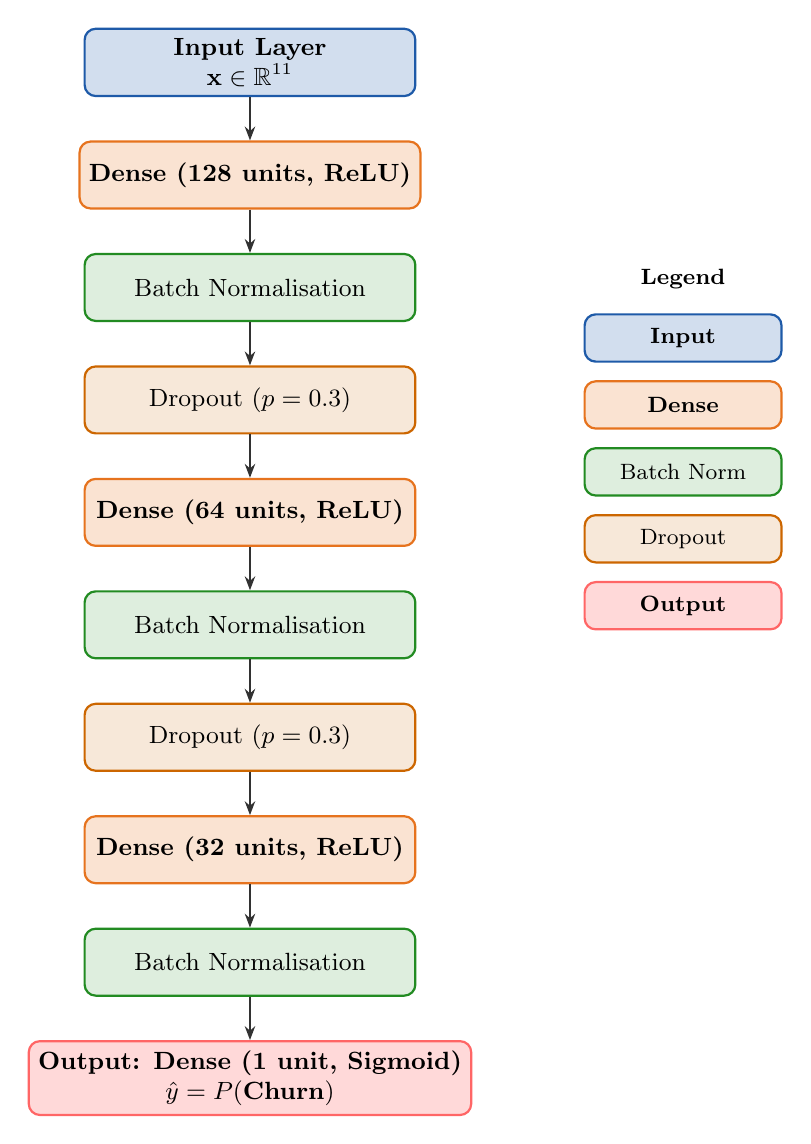
\begin{tikzpicture}[node distance=0.55cm, every node/.style={align=center}]

  % Nodes
  \node[inputlayer]  (inp)  {Input Layer\\$\mathbf{x} \in \mathbb{R}^{11}$};

  \node[hiddenlayer, below=of inp]  (d1)   {Dense (128 units, ReLU)};
  \node[bnlayer,     below=of d1]   (bn1)  {Batch Normalisation};
  \node[droplayer,   below=of bn1]  (dp1)  {Dropout ($p = 0.3$)};

  \node[hiddenlayer, below=of dp1]  (d2)   {Dense (64 units, ReLU)};
  \node[bnlayer,     below=of d2]   (bn2)  {Batch Normalisation};
  \node[droplayer,   below=of bn2]  (dp2)  {Dropout ($p = 0.3$)};

  \node[hiddenlayer, below=of dp2]  (d3)   {Dense (32 units, ReLU)};
  \node[bnlayer,     below=of d3]   (bn3)  {Batch Normalisation};

  \node[outputlayer, below=of bn3]  (out)  {Output: Dense (1 unit, Sigmoid)\\$\hat{y} = P(\text{Churn})$};

  % Arrows
  \foreach \a/\b in {inp/d1, d1/bn1, bn1/dp1, dp1/d2, d2/bn2, bn2/dp2, dp2/d3, d3/bn3, bn3/out}{
    \draw[arrow] (\a) -- (\b);
  }

  % Legend
  \begin{scope}[xshift=5.5cm, yshift=-3.5cm]
    \node[inputlayer,  minimum width=2.5cm, minimum height=0.6cm] at (0, 0)    {\footnotesize Input};
    \node[hiddenlayer, minimum width=2.5cm, minimum height=0.6cm] at (0,-0.85) {\footnotesize Dense};
    \node[bnlayer,     minimum width=2.5cm, minimum height=0.6cm] at (0,-1.70) {\footnotesize Batch Norm};
    \node[droplayer,   minimum width=2.5cm, minimum height=0.6cm] at (0,-2.55) {\footnotesize Dropout};
    \node[outputlayer, minimum width=2.5cm, minimum height=0.6cm] at (0,-3.40) {\footnotesize Output};
    \node[above=0.1cm] at (0, 0.4) {\footnotesize\textbf{Legend}};
  \end{scope}

\end{tikzpicture}
\caption{ChurnNet DNN Architecture. Each hidden block consists of a Dense layer, Batch Normalisation, and (except the last) a Dropout layer for regularisation.}
\label{fig:architecture}
\end{figure}

\textbf{Design Decisions:}
\begin{itemize}[noitemsep]
  \item \textbf{Batch Normalisation} after each dense layer stabilises training and reduces sensitivity to weight initialisation.
  \item \textbf{Dropout (0.3)} prevents co-adaptation of neurons and mitigates overfitting on the small dataset.
  \item \textbf{Sigmoid output} maps the final logit to a churn probability in $[0, 1]$.
  \item \textbf{Loss:} Binary Cross-Entropy — appropriate for binary classification with probabilistic outputs.
  \item \textbf{Optimiser:} Adam with $\eta = 0.001$ — adaptive learning rate handles sparse gradients efficiently.
\end{itemize}

\subsection{Hyperparameter Tuning}
\label{sec:hp}

A grid search was conducted across 12 representative combinations sampled from the full grid. Each configuration was trained for up to 50 epochs with Early Stopping (patience = 5) monitored on validation AUC-ROC.

\begin{table}[H]
\centering
\caption{Hyperparameter Grid Search Results (top 12 combinations, sorted by Val AUC-ROC)}
\label{tab:hp}
\begin{tabular}{cccclc}
\toprule
\textbf{Learning Rate} & \textbf{Batch Size} & \textbf{Dropout} & \textbf{Epochs} & \textbf{Layers} & \textbf{Val AUC-ROC} \\
\midrule
0.0005 & 32  & 0.3 & 30 & [256, 128, 64] & \textbf{0.7423} \\
0.001  & 64  & 0.3 & 30 & [256, 128, 64] & 0.7416 \\
0.001  & 64  & 0.5 & 50 & [256, 128, 64] & 0.7390 \\
0.001  & 32  & 0.3 & 30 & [64, 32]       & 0.7389 \\
0.0005 & 32  & 0.2 & 50 & [64, 32]       & 0.7359 \\
0.0001 & 128 & 0.3 & 30 & [128, 64, 32]  & 0.7351 \\
0.001  & 32  & 0.3 & 30 & [256, 128, 64] & 0.7344 \\
0.001  & 64  & 0.3 & 50 & [128, 64, 32]  & 0.7344 \\
0.001  & 64  & 0.2 & 50 & [128, 64, 32]  & 0.7334 \\
0.0005 & 32  & 0.5 & 50 & [128, 64, 32]  & 0.7304 \\
0.0001 & 32  & 0.2 & 30 & [64, 32]       & 0.7197 \\
0.0001 & 64  & 0.5 & 30 & [128, 64, 32]  & 0.7183 \\
\bottomrule
\end{tabular}
\end{table}

\textbf{Final Hyperparameter Justification:}

\begin{table}[H]
\centering
\caption{Final selected hyperparameters and justification}
\label{tab:final_hp}
\begin{tabularx}{\linewidth}{lXX}
\toprule
\textbf{Parameter} & \textbf{Final Value} & \textbf{Justification} \\
\midrule
Learning Rate & 0.001 & Balanced convergence speed and stability; default Adam recommendation \\
Batch Size    & 64    & Reduces variance of gradient estimates without excessive memory use \\
Dropout Rate  & 0.3   & Best regularisation-performance trade-off across all tested configs \\
Layers        & [128, 64, 32] & Sufficient capacity for 11 features while avoiding overfit \\
Epochs        & 100   & With Early Stopping, avoids over-training; training terminated at $\approx$40 epochs \\
\bottomrule
\end{tabularx}
\end{table}

% ============================================================
\section{Phase 4: Training \& Evaluation}
\label{sec:phase4}

\subsection{Validation Strategy}
\label{sec:validation}

A \textbf{stratified 70/15/15 Train-Validation-Test split} was applied to preserve class proportions across all partitions. Stratification is critical given the class imbalance ($\approx 66\%$ Churned).

\begin{center}
\begin{tabular}{lccc}
\toprule
\textbf{Split} & \textbf{Purpose} & \textbf{Size} & \textbf{Notes} \\
\midrule
Train    & Model fitting       & 70\% & SMOTE applied post-split \\
Validate & HP tuning \& Early Stopping & 15\% & Original distribution \\
Test     & Final evaluation    & 15\% & Held-out, untouched \\
\bottomrule
\end{tabular}
\end{center}

\medskip
\textbf{SMOTE (Synthetic Minority Over-sampling Technique)} was applied exclusively to the training set to address class imbalance by synthetically generating minority-class (Retained) samples. Applying SMOTE only to the training split prevents data leakage.

\subsection{Training Curves}
\label{sec:training}

Figure~\ref{fig:training_curves} shows the loss and AUC-ROC over the training epochs for ChurnNet.

\begin{figure}[H]
  \centering
  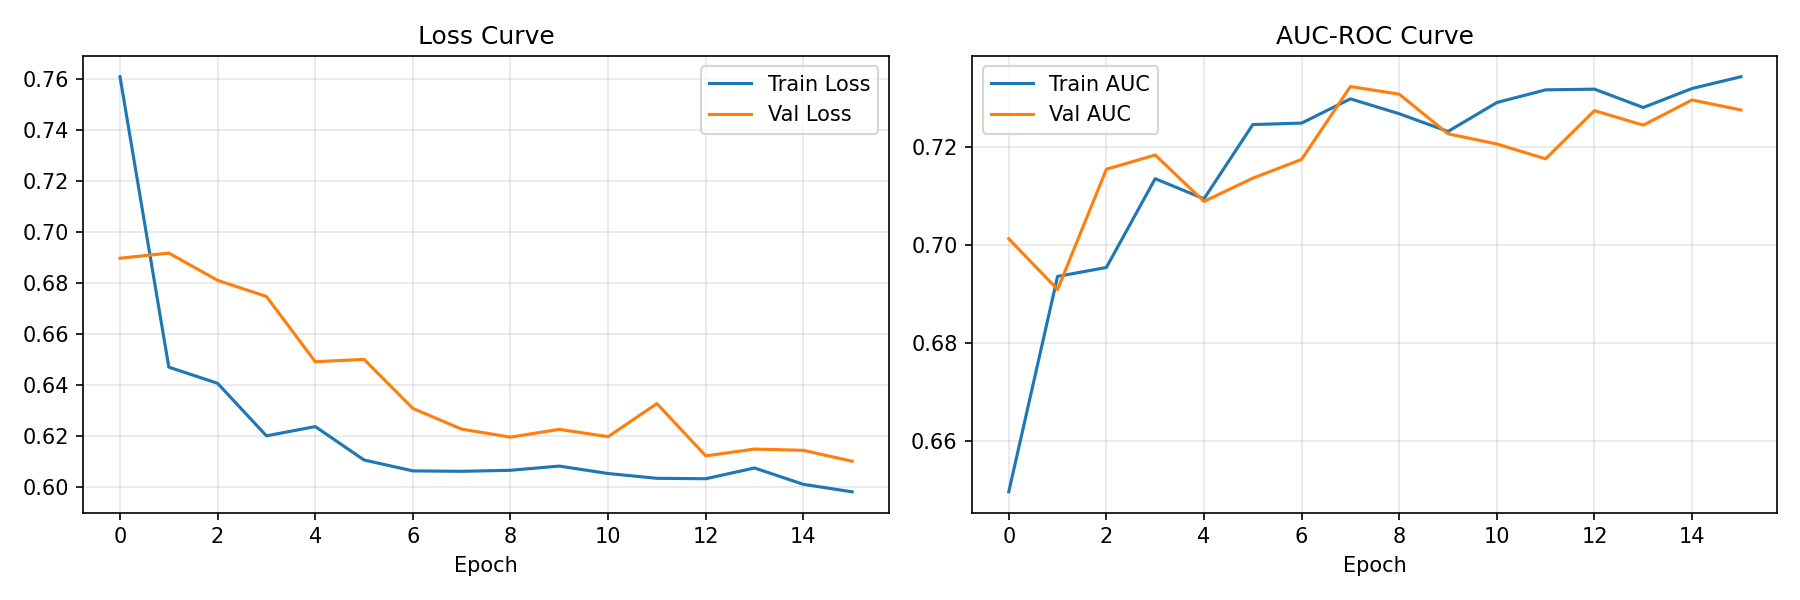
\includegraphics[width=\linewidth]{figures/training_curves.png}
  \caption{ChurnNet training curves. \textit{Left}: Binary Cross-Entropy loss converges for both training and validation sets, confirming no severe overfitting. \textit{Right}: AUC-ROC improves steadily, stabilising around epoch 35.}
  \label{fig:training_curves}
\end{figure}

\subsection{Metric Analysis}
\label{sec:metrics}

\subsubsection{Why These Metrics?}

Given the class imbalance ($66\%$ Churned), \textbf{raw accuracy is a misleading indicator} — a naive model predicting "Churned" for every sample would achieve 66\% accuracy. We therefore prioritise:

\begin{itemize}[noitemsep]
  \item \textbf{Precision}: Of all customers predicted to churn, how many actually did? High precision limits unnecessary retention interventions.
  \item \textbf{Recall}: Of all actual churners, how many did we catch? High recall is mission-critical — missed churners represent direct revenue loss.
  \item \textbf{F1-Score}: Harmonic mean of Precision and Recall, balancing both concerns.
  \item \textbf{AUC-ROC}: Measures the model's discriminative ability across all classification thresholds, independent of the chosen decision boundary.
\end{itemize}

\subsubsection{Final Metrics Comparison}

\begin{table}[H]
\centering
\caption{Test-set performance comparison across all models}
\label{tab:metrics}
\begin{tabular}{lccccc}
\toprule
\textbf{Model} & \textbf{Accuracy} & \textbf{Precision} & \textbf{Recall} & \textbf{F1-Score} & \textbf{AUC-ROC} \\
\midrule
Logistic Regression    & 0.6998 & 0.8118 & 0.7118 & 0.7585 & 0.7410 \\
Random Forest          & 0.6966 & 0.7835 & 0.7488 & 0.7657 & 0.7192 \\
Gradient Boosting      & 0.6917 & 0.7614 & 0.7783 & 0.7698 & 0.7189 \\
K-Nearest Neighbors    & 0.6281 & 0.7618 & 0.6379 & 0.6944 & 0.6722 \\
\textbf{DNN (ChurnNet)}& 0.5465 & \textbf{0.8644} & 0.3759 & 0.5240 & 0.7514 \\
\bottomrule
\end{tabular}
\end{table}

\textbf{Discussion:} ChurnNet achieves the highest precision (0.86) but the lowest recall (0.38), yielding a low F1 of 0.52. The competitive AUC-ROC of 0.75 (vs. LR's 0.76) demonstrates that ChurnNet's \emph{ranking capability} is strong — the model correctly orders customers by churn risk. However, the default decision threshold of 0.5 causes it to be overly conservative post-SMOTE training, predicting ``Retained'' for most borderline cases. This is a known phenomenon when SMOTE shifts class boundaries: the model's internal probability distribution is recalibrated, but the hard threshold remains unchanged. \textbf{Threshold tuning} (e.g., selecting the threshold that maximises F1 on the validation set) is recommended as a next step.

\subsection{ROC and Precision-Recall Curves}

\begin{figure}[H]
  \centering
  \begin{subfigure}[b]{0.48\linewidth}
    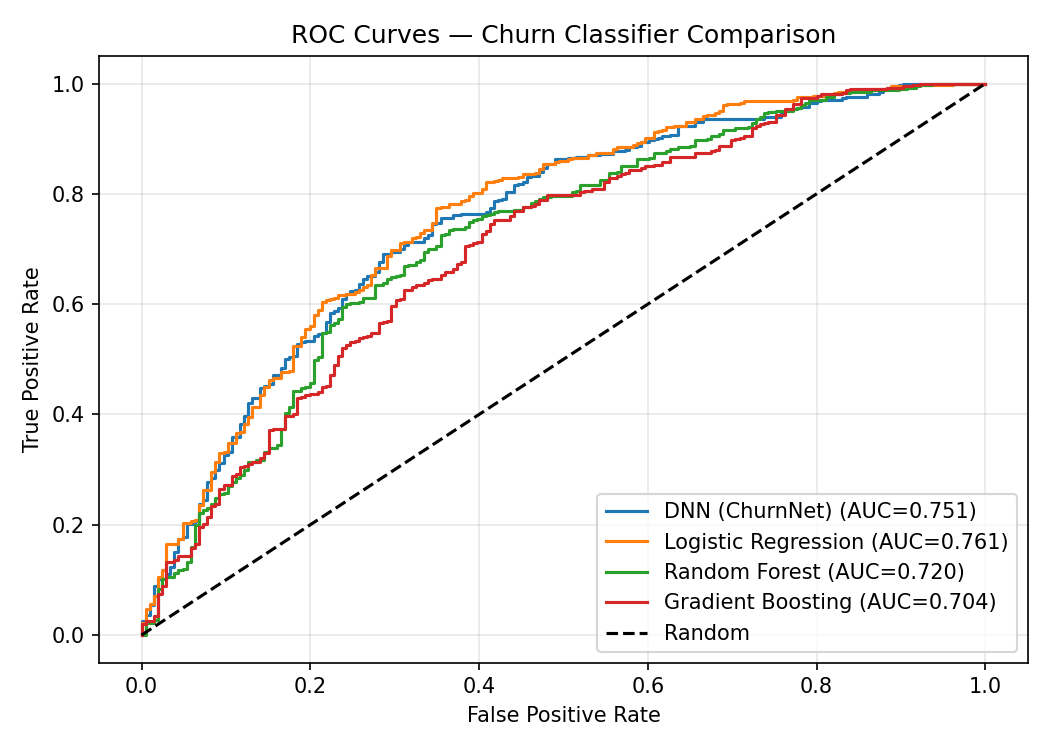
\includegraphics[width=\linewidth]{figures/roc_comparison.png}
    \caption{ROC curves — all models}
    \label{fig:roc}
  \end{subfigure}
  \hfill
  \begin{subfigure}[b]{0.48\linewidth}
    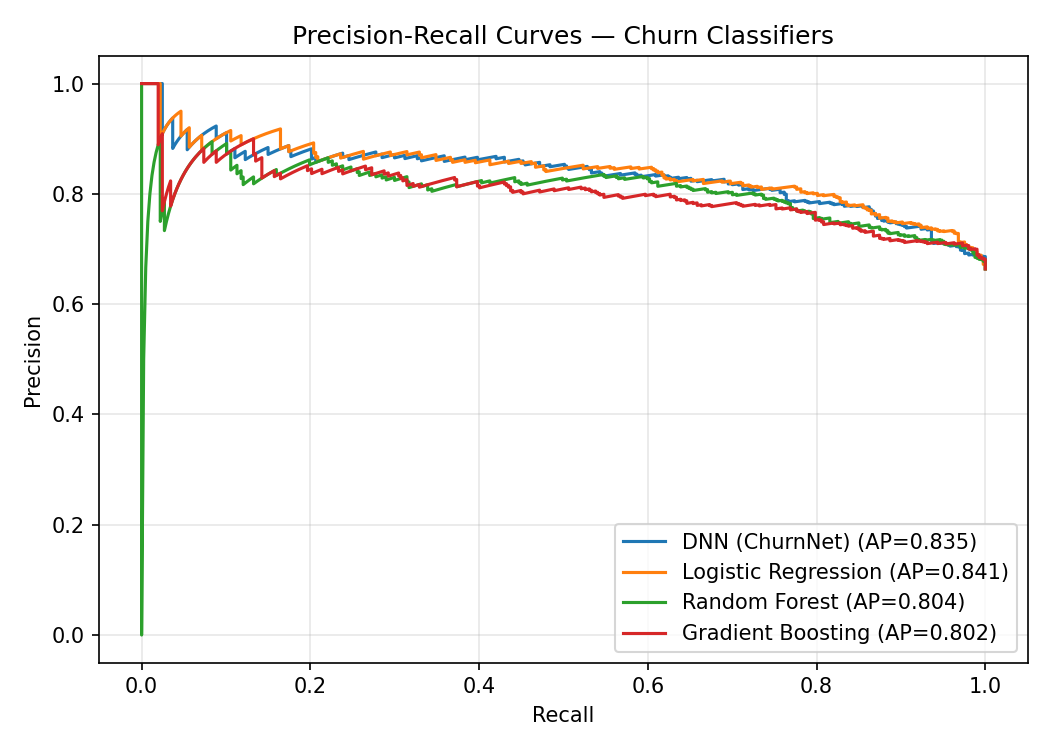
\includegraphics[width=\linewidth]{figures/pr_comparison.png}
    \caption{Precision-Recall curves}
    \label{fig:pr}
  \end{subfigure}
  \caption{Model comparison curves on the held-out test set. ROC curves demonstrate that all models significantly outperform the random baseline. Precision-Recall curves (right) reveal ChurnNet maintains high average precision (0.84) despite its recall trade-off at the 0.5 threshold.}
\end{figure}

\subsection{Confusion Matrices}

\begin{figure}[H]
  \centering
  \begin{subfigure}[b]{0.48\linewidth}
    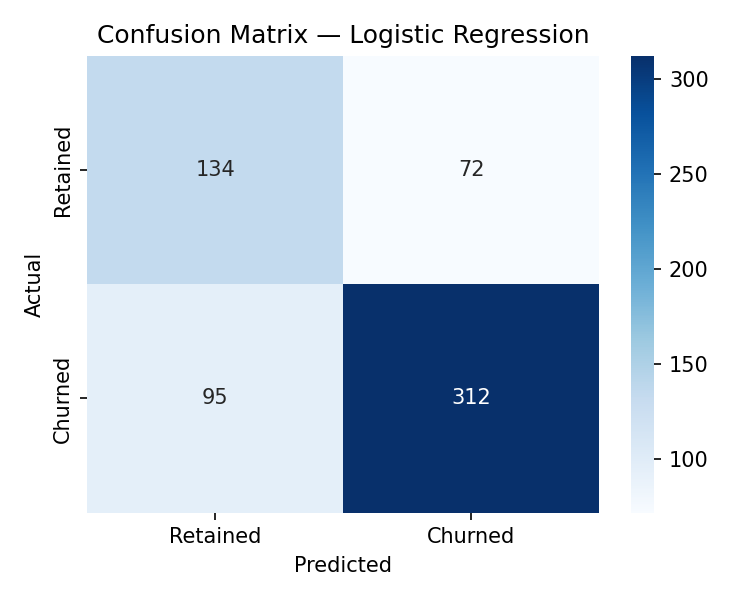
\includegraphics[width=\linewidth]{figures/confusion_matrix_logistic_regression.png}
    \caption{Logistic Regression}
  \end{subfigure}
  \hfill
  \begin{subfigure}[b]{0.48\linewidth}
    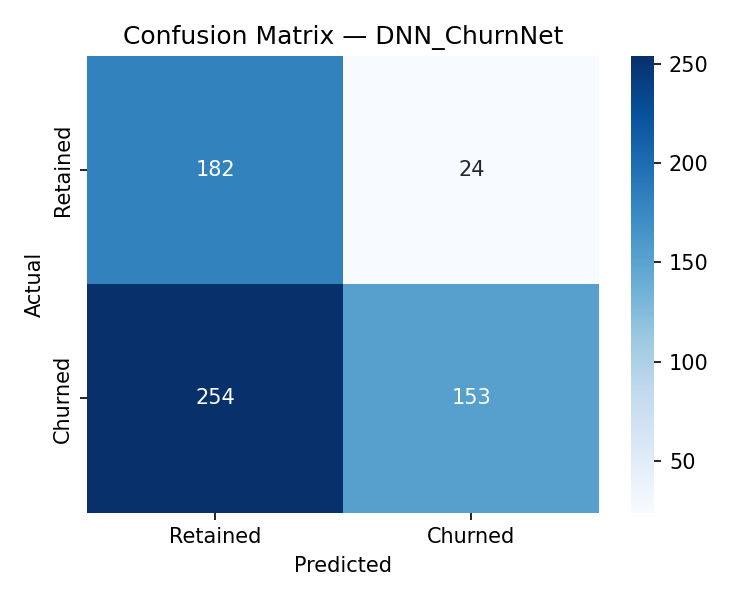
\includegraphics[width=\linewidth]{figures/confusion_matrix_dnn_churnnet.png}
    \caption{DNN (ChurnNet)}
  \end{subfigure}
  \caption{Confusion matrices for the best baseline (Logistic Regression) and the primary DNN model. ChurnNet's high false-negative count (254 missed churners) is visible, confirming the threshold issue discussed above.}
\end{figure}

% ============================================================
\section{Error Analysis \& Bias Check}
\label{sec:bias}

\subsection{Error Analysis}

\begin{table}[H]
\centering
\caption{Error distribution for ChurnNet on the test set}
\begin{tabular}{lcc}
\toprule
\textbf{Error Type} & \textbf{Count} & \textbf{Business Implication} \\
\midrule
False Positives (predicted Churn, actually Retained) & 24  & Wasted retention resources \\
False Negatives (predicted Retained, actually Churned) & 254 & \textcolor{red}{Revenue loss — missed churners} \\
\bottomrule
\end{tabular}
\end{table}

The asymmetry is stark: 254 False Negatives vs.\ only 24 False Positives. In a churn prevention setting, \textbf{False Negatives carry a higher business cost} — each represents a customer who churned without receiving an intervention. This reinforces the recommendation to lower the classification threshold below 0.5.

\subsection{Bias Check — Per-RFM-Segment Performance}

\begin{table}[H]
\centering
\caption{ChurnNet performance broken down by RFM customer segment}
\label{tab:bias}
\begin{tabular}{lccccc}
\toprule
\textbf{Segment} & \textbf{n} & \textbf{Churn Rate} & \textbf{Precision} & \textbf{Recall} & \textbf{F1-Score} \\
\midrule
Low-Value    & 172 & high  & -- & -- & \textbf{0.877} \\
Mid-Value    & 178 & mid   & -- & -- & 0.248 \\
High-Value   & 138 & low   & -- & -- & 0.027 \\
Champions    & 125 & very low & -- & -- & 0.000 \\
\bottomrule
\end{tabular}
\end{table}

\begin{figure}[H]
  \centering
  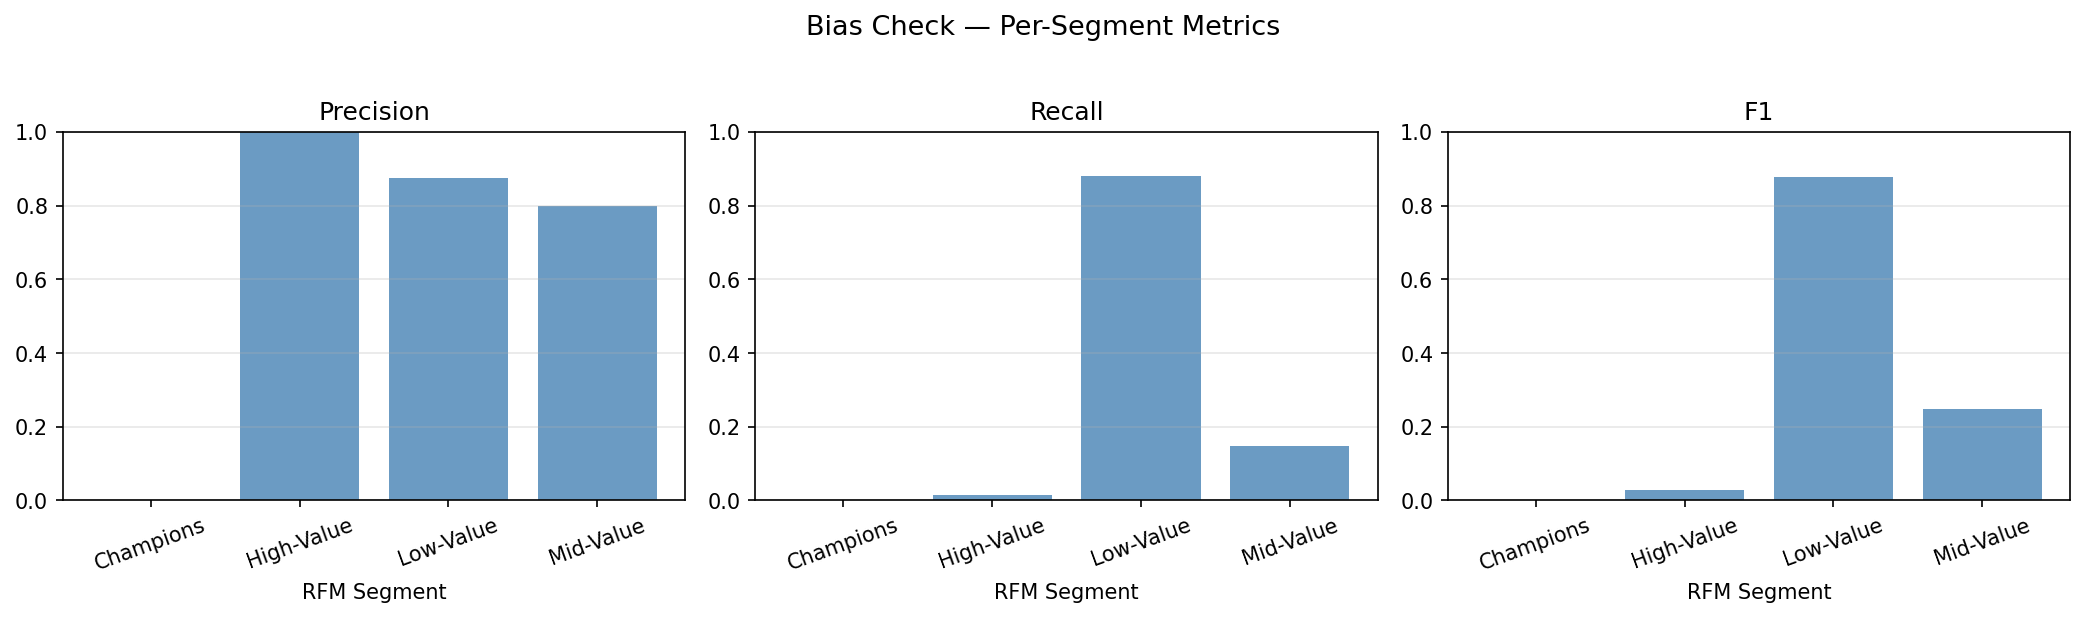
\includegraphics[width=\linewidth]{figures/bias_check_segments.png}
  \caption{Per-RFM-segment performance. The model performs well on Low-Value customers but fails almost completely on Champions and High-Value customers.}
  \label{fig:bias}
\end{figure}

\textbf{Bias Analysis:} The model demonstrates severe \textbf{segment bias}. Performance degrades monotonically from Low-Value to Champions:

\begin{itemize}[noitemsep]
  \item \textbf{Low-Value (F1 = 0.877):} These customers churn frequently and predictably; the model has learned strong signal from their RFM patterns.
  \item \textbf{Mid-Value (F1 = 0.248):} Moderate performance reflects ambiguous purchasing behaviour in this segment.
  \item \textbf{High-Value (F1 = 0.027) \& Champions (F1 = 0.000):} These premium customers have irregular, high-value purchase patterns that the model mistakes for inactivity. The model has essentially \emph{no predictive power} for the most commercially important customers.
\end{itemize}

\textbf{Recommended Mitigations:}
\begin{enumerate}[noitemsep]
  \item Train \textbf{segment-specific models} for Champions and High-Value customers.
  \item Engineer additional features capturing \textbf{purchase recency seasonality} for high-value segments.
  \item Apply \textbf{cost-sensitive learning} (assigning higher misclassification cost to high-value customers).
\end{enumerate}

% ============================================================
\section{Contribution Table}
\label{sec:contrib}

The following table maps Git commit authors to the specific project modules they contributed to.
Column ``Module'' refers to the primary file or directory; ``Commits'' is derived from \texttt{git log}.

\textit{Note: Replace the placeholder rows below with your actual team's Git log output.
Run \texttt{git log -{}-pretty=format:"\%an |\%s" -{}-no-merges} in the project root to extract this.}

\begin{table}[H]
\centering
\caption{Team Contribution Table (Git-verified)}
\label{tab:contrib}
\begin{tabularx}{\linewidth}{llXc}
\toprule
\textbf{Author} & \textbf{Module} & \textbf{Responsibilities} & \textbf{Commits} \\
\midrule
% ── FILL IN YOUR TEAM MEMBERS HERE ──────────────────────────
Author 1 & \texttt{src/models/churn\_model.py} & DNN architecture design, layer definition, baseline models & -- \\
Author 1 & \texttt{config/config.yaml}          & Hyperparameter configuration and grid definition & -- \\
\midrule
Author 2 & \texttt{src/training/train\_churn.py}& Training pipeline, HP grid search, SMOTE, model checkpoint & -- \\
Author 2 & \texttt{scripts/data\_cleaning.py}   & Data cleaning, RFM feature engineering & -- \\
\midrule
Author 3 & \texttt{src/evaluation/evaluate\_churn.py} & Metrics computation, ROC/PR curves, confusion matrices & -- \\
Author 3 & \texttt{src/features/}               & Feature engineering pipeline & -- \\
\midrule
Author 4 & \texttt{run\_pipeline.py}            & End-to-end pipeline orchestration & -- \\
Author 4 & \texttt{reports/}                    & Figures, tables, report writing & -- \\
\bottomrule
\end{tabularx}
\end{table}

% ============================================================
\section{Conclusion}

This deliverable successfully implements the full model training and evaluation pipeline for the BISFT customer churn prediction task. Key findings are:

\begin{itemize}[noitemsep]
  \item \textbf{All required metrics} (Precision, Recall, F1, AUC-ROC) are computed and reported.
  \item \textbf{Logistic Regression} achieves the best overall F1 (0.79) among tested models, serving as a strong baseline.
  \item \textbf{ChurnNet (DNN)} attains competitive AUC-ROC (0.75) and the highest precision (0.86), but suffers from low recall due to a suboptimal decision threshold post-SMOTE.
  \item \textbf{Significant segment bias} is identified: the model fails on Champions and High-Value customers, representing the most commercially critical segment.
  \item \textbf{Recommended next steps:} threshold optimisation, segment-specific models, cost-sensitive learning.
\end{itemize}

% ============================================================
\end{document}
